\documentclass[11pt, oneside]{article} 
\usepackage{geometry}
\geometry{letterpaper} 
\usepackage{graphicx}
	
\usepackage{amssymb}
\usepackage{amsmath}
\usepackage{parskip}
\usepackage{color}
\usepackage{hyperref}

\graphicspath{{/Users/telliott/Github/precalculus/fig/}}

\title{Congruence of triangles}
\date{}

\begin{document}
\maketitle
\Large

\subsection*{congruence}

\textcolor{red}{
$\bullet$  Two triangles are \emph{congruent} if and only if they have the same three side lengths.} 

Congruence is a fancy word for equal.  The condition we use is often abbreviated SSS (side-side-side). 

By this definition, a triangle and its mirror image are congruent.  The three triangles shown below are all congruent, even though two are flipped (they are mirror images).

\begin{center} 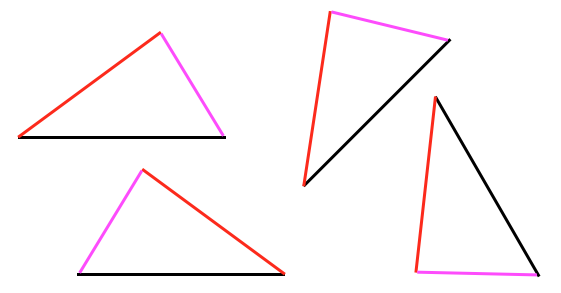
\includegraphics [scale=0.4] {congruent.png} \end{center}

Having three sides equal means that the shape is the same.  The three angles are also equal --- and the shapes are superimposable, with the proviso that we allow the shape to be flipped over.

In addition to SSS (side-side-side), there are three other conditions that lead to congruence of two triangles when they are satisfied, namely

$\circ$  SAS (side-angle-side)

$\circ$  ASA (angle-side-angle)

$\circ$  AAS (angle-angle-side)

\subsection*{similarity}

\textcolor{red}{Some triangles are \emph{similar} but not congruent.}

Similarity means that the three angles are the same but the triangles are of different overall sizes.  

We might say that they are the same but \emph{scaled} differently.  

We call this AAA (angle-angle-angle).  For similar triangles, the three corresponding pairs of sides are in the same proportions, but re-scaled by a constant of proportion.

\textcolor{red}{$\bullet$  Two triangles are similar if they have at least two angles equal.}

Because of the triangle sum theorem (\hyperref[sec:triangle_sum_theorem]{\textbf{ref}}), if any two angles of a pair of triangles are known to be equal, then the third one must be equal as well.

Similar triangles have their sides in the same proportion.  This is known as the AAA similarity theorem.

\begin{center} 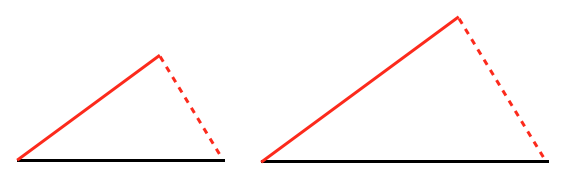
\includegraphics [scale=0.4] {similar.png} \end{center}

Given any triangle, draw a line parallel to one side, which also joins the other two sides.  The new triangle with that side as its base is similar to the given triangle.

\begin{center} 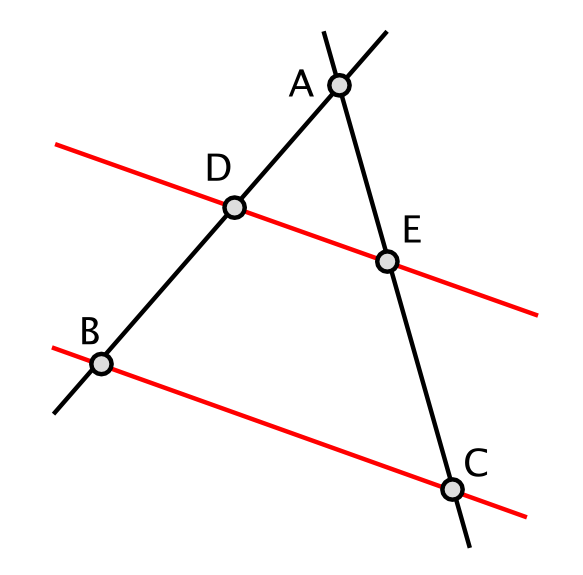
\includegraphics [scale=0.25] {Thales_theorem_1.png} \end{center}

In this example, these ratios are equal
\[ \frac{AD}{AB} = \frac{AE}{AC} = \frac{DE}{BC}  \]
and you can find others.

Statements about similarity:

$\circ$ \ similar triangles have all three angles equal 

$\circ$ \ if two similar triangles are superimposed, the two sides that do not coincide with each other, are parallel

$\circ$ \ similar triangles have their similar sides in the same ratio
  
It is easy to see why the first two statements are equivalent.  Just use the alternate interior angles theorem.

The third is harder.  For now we will assume the theorem:  that AAA and sides in proportion are both the same as similarity.

\subsection*{constructions}

The way I think about the congruence conditions is to imagine trying to construct a triangle from the given information, and ask whether it is uniquely determined.  Suppose we know ASA.  The situation is thus:

\begin{center} 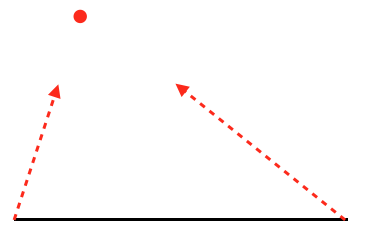
\includegraphics [scale=0.4] {ASA1.png} \end{center}
 
Draw the known side, then using the known angles, start two other sides from the ends of that side.  They must cross at a unique point.  

But... actually, if we start the two lines from opposite ends of the horizontal

\begin{center} 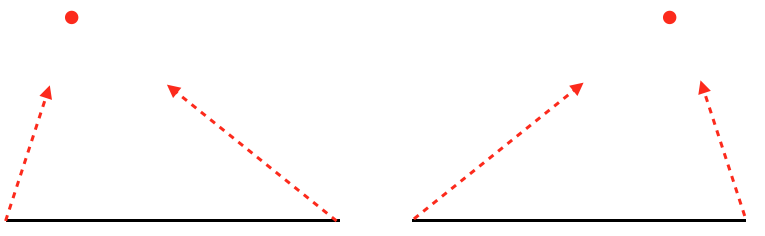
\includegraphics [scale=0.4] {ASA4.png} \end{center}

there is another solution, the mirror image.  These two triangles are congruent to the one above.
 
I'm tempted to add still another:

\begin{center} 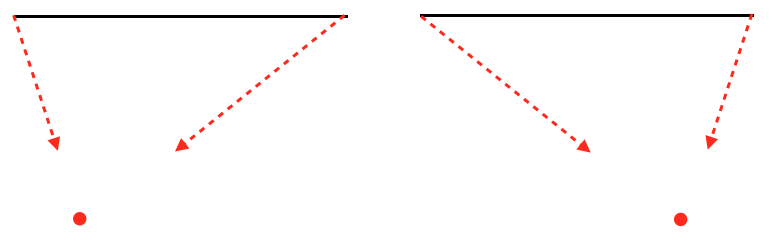
\includegraphics [scale=0.4] {ASA5.png} \end{center}

But this doesn't give anything new.  These are merely rotated versions of the ones above.  Congruent triangles include the two mirror images and that's it.

If we know two angles we also know the third, because they must add to 180 degrees.  For this reason, ASA and AAS imply that we have exactly the same information, because we know all three angles and we know one side.  

This restriction is crucial:  we must also know \emph{which} two angles flank the known side.  Alternatively, it is enough to know which angle is opposite to the known side.
 
\subsection*{SAS, ASA, AAS but not SSA}

SAS is very commonly used to prove congruence.  
\begin{center} 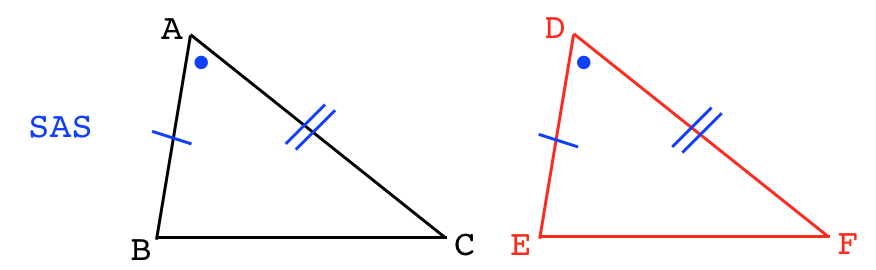
\includegraphics [scale=0.4] {SAS.png} \end{center}

In this diagram, sides of equal length are indicated by one or more hash marks.  

Equal angles are usually indicated by dots in this book. (Dots are easier to place on the figures, and lend themselves to color-coding;  the common method for pencil and paper is to draw an arc with a hash across it).

The other methods for proving congruence use two equal angles and a side.  Two equal angles imply the third angle is also equal (since they add to a half-circle or 180 degrees), so the two triangles are similar.  To prove they are congruent, we need one side.

These methods using two angles are referred to as ASA
\begin{center} 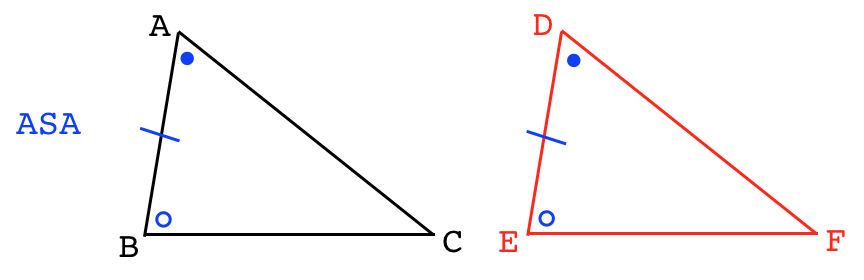
\includegraphics [scale=0.4] {ASA3.png} \end{center}

 and AAS.
\begin{center} 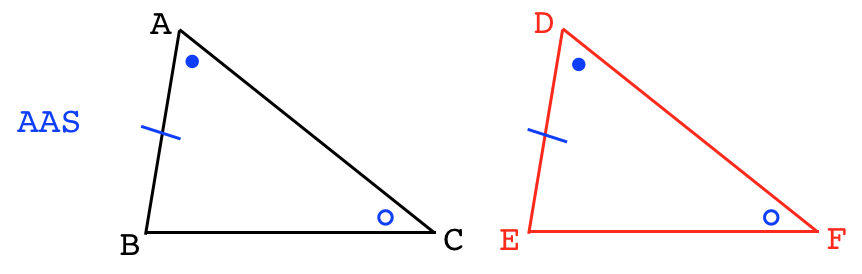
\includegraphics [scale=0.4] {AAS.png} \end{center}

Because AA implies AAA, these tell unambiguously which angle is opposite the known side.

\subsection*{one that works only sometimes}

There is one set of three that doesn't work in the general case, that is SSA (side-side-angle).

\begin{center} 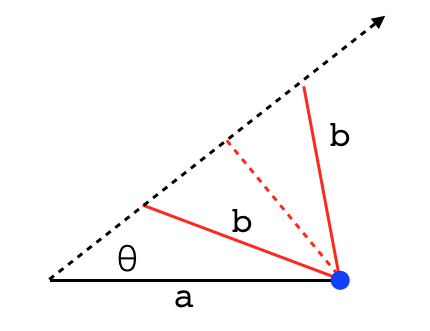
\includegraphics [scale=0.4] {angle_side_side.png} \end{center}

Here we know sides $a$ and $b$ and the angle $\theta$ adjacent to $a$ and facing opposite side $b$.  Imagine $b$ swinging on a hinge at the blue dot.  If $b < a$, there are two points where $b$ can intersect with the side projecting from angle $\theta$.  There is no unique solution, so the triangle is not determined.

On the other hand, if

$\circ$ \ $b > a$, or alternatively 

$\circ$ \ $b = a$, in which case the triangle is isosceles and we have two angles plus two sides

$\circ$ \ $b$ forms a right angle with the third side, in which case we also have two angles

then the triangle \emph{would} be determined.

There is a temptation to call this case ASS.  I think Tony Randall said it best:

\url{https://www.youtube.com/watch?v=KEP1acj29-Y}



\end{document}